%% =====================================================================
%%  Electromagnetismo I · Tema 6 · Teoría del potencial (Parte I)
%%  ESQUEMA SIMBÓLICO: desarrollos encadenados con comentario mínimo,
%%  pensado como guion para los apuntes manuscritos.
%%  Compilar con:  pdflatex (dos pasadas)  ·  latexmk -pdf
%% =====================================================================
\documentclass[11pt,a4paper,twoside]{article}
\usepackage{estilo/tema6-estilo}
\renewcommand{\cabeceraTema}{Tema 6 \textperiodcentered{} Esquema simbólico}

\hypersetup{pdftitle={Tema 6. Teoría del potencial (Parte I). Esquema simbólico},
            pdfauthor={Daniel Martín Guerrero},
            pdfsubject={Electromagnetismo I}}

% Paso numerado de un desarrollo: \paso{título}
\newcounter{paso}[section]
\newcommand{\paso}[1]{\par\smallskip\refstepcounter{paso}\noindent
  {\color{azul}\bfseries\thepaso.\ }{\color{celeste}\itshape #1}\par\nopagebreak\smallskip}
% Comentario breve al margen de una cadena de igualdades
\newcommand{\com}[1]{\quad{\color{gristexto}\footnotesize\text{#1}}}

\begin{document}

%% ------------------------------------------------------------- CABECERA
\thispagestyle{plain}
\begin{center}
  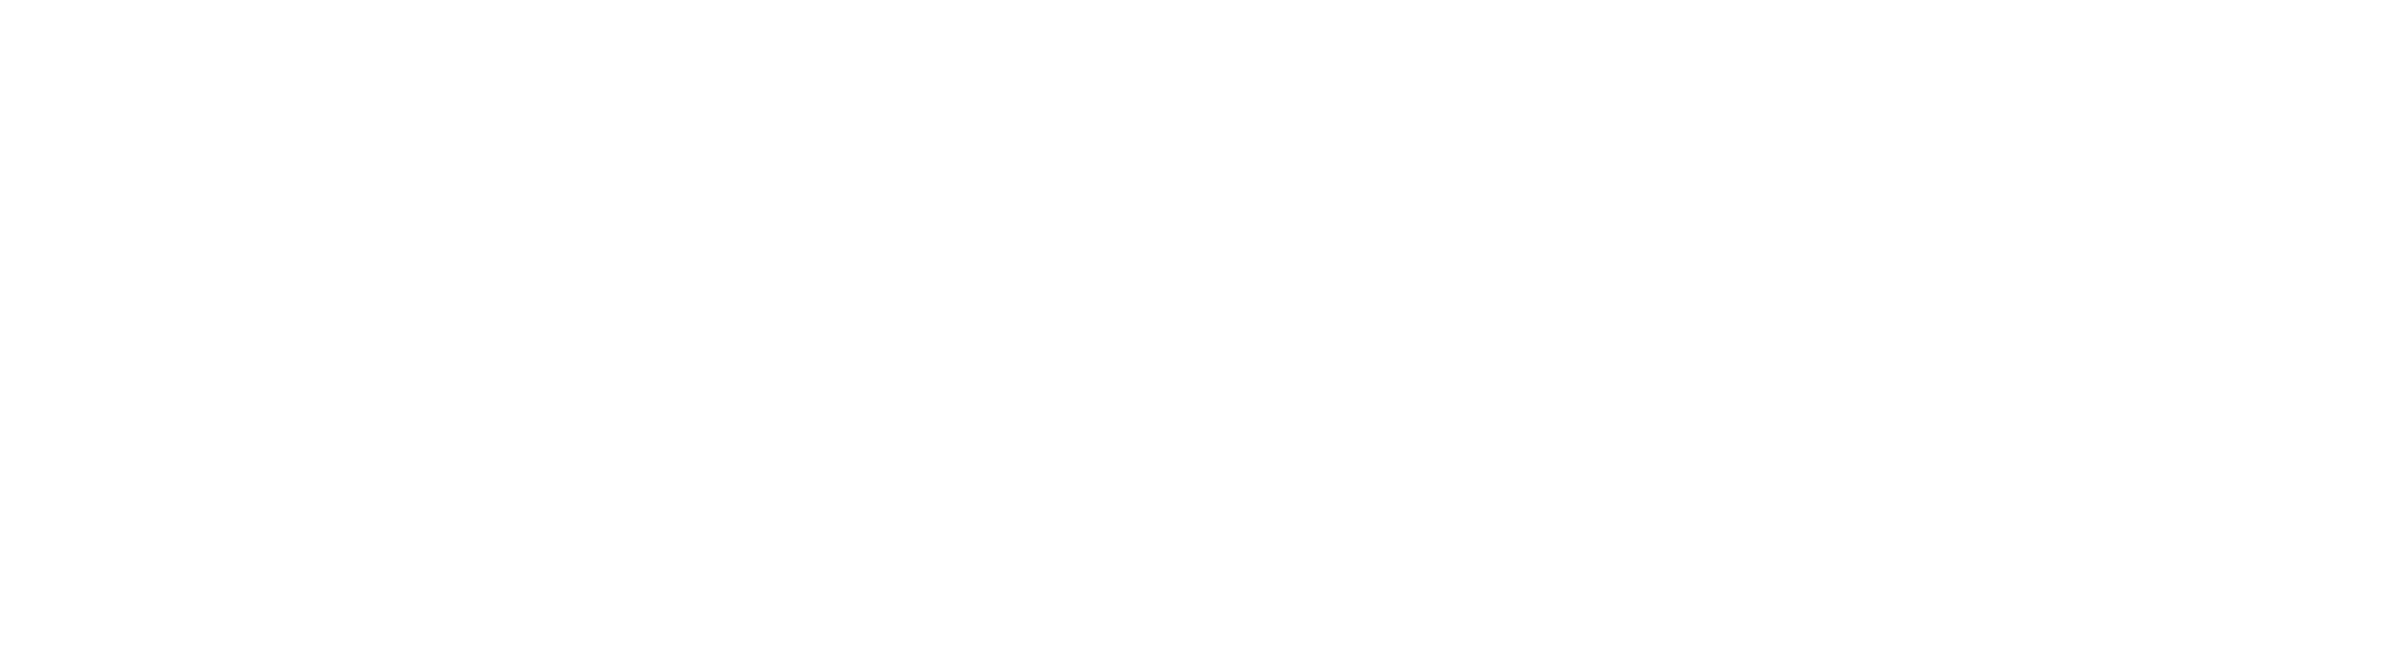
\includegraphics[width=3.4cm]{estilo/logo-usal.png}\par\vspace{0.3cm}
  {\color{gristexto}\rule{\textwidth}{0.4pt}}\par\vspace{0.2cm}
  {\color{azul}\textsc{Electromagnetismo I}}\quad{\color{gristexto}\textperiodcentered\quad\textsc{Tema 6 \textperiodcentered{} Parte I}}\par
  \vspace{0.25cm}
  {\fontsize{22}{26}\selectfont\bfseries Teoría del potencial}\par\vspace{0.1cm}
  {\color{gristexto}\itshape Esquema simbólico: desarrollos completos con comentario mínimo}\par
  \vspace{0.2cm}{\color{gristexto}\rule{\textwidth}{0.4pt}}
\end{center}

\begin{nota}{Notación}
$\vR=\vr-\vrp$, $R=\abs{\vR}$, $\uR=\vR/R$; primas: derivadas respecto de $\vrp$;
$\dd\bm S=\un\dS$ ($\un$ exterior), $\partial_n=\un\cdot\nablav$; medio lineal isótropo
$\eps(\vr)>0$; $\rho\equiv\rhof$.
\end{nota}

\setcounter{tocdepth}{1}
{\small\tableofcontents}

%% =====================================================================
\section{Poisson y Laplace}
%% =====================================================================

\paso{Ecuación de Poisson generalizada}
\begin{equation}
  \rot\vE=\bm0\ \implica{Stokes}\ \vE=-\nablav\varphi,\qquad
  \nablav\cdot\vD=\rho,\quad\vD=\eps\vE
  \ \implica{}\ \caja{\nablav\cdot(\eps\nablav\varphi)=-\rho}
\end{equation}
\begin{equation}
  \nablav\cdot(\eps\nablav\varphi)=\nablav\eps\cdot\nablav\varphi+\eps\lap\varphi=-\rho
  \ \implica{}\
  \lap\varphi=-\frac1\eps\bigl(\rho+\nablav\eps\cdot\nablav\varphi\bigr)
\end{equation}

\paso{Medio homogéneo}
\begin{equation}
  \nablav\eps=\bm0:\qquad \lap\varphi=-\frac{\rho}{\eps}
  \quad\bigl(\text{vacío: }-\rho/\epsz\bigr),\qquad
  \rho=0:\ \caja{\lap\varphi=0}
\end{equation}

\paso{La función $1/R$}
\begin{gather}
  \nablav\frac1R=-\frac{\uR}{R^{2}},\qquad\gradp\frac1R=+\frac{\uR}{R^{2}},\qquad
  \nablav\cdot\frac{\vR}{R^{3}}=\frac{3}{R^{3}}-\frac{3R^{2}}{R^{5}}=0\ \ (R\neq0)\\
  \int_{B_\epsilon}\lap\frac1R\dV=\oint_{\partial B_\epsilon}\Bigl(-\frac{\uR}{R^{2}}\Bigr)\cdot\uR R^{2}\dd\Omega=-4\pi
  \ \implica{}\ \caja{\lap\frac1R=\lapp\frac1R=-4\pi\delta^{3}(\vr-\vrp)}
\end{gather}

\paso{Todas las fuentes conocidas}
\begin{equation}
  \varphi(\vr)=\frac{1}{4\pi\epsz}\int\frac{\rho(\vrp)}{\abs{\vr-\vrp}}\dVp
  \ \implica{}\
  \lap\varphi=\frac{1}{4\pi\epsz}\int\rho(\vrp)\bigl[-4\pi\delta^{3}(\vr-\vrp)\bigr]\dVp=-\frac{\rho(\vr)}{\epsz}
\end{equation}

\paso{Laplace en 1D}
\begin{equation}
  \varphi''=0\implica{}\varphi=Ax+B,\qquad
  \tfrac12\bigl[\varphi(x+a)+\varphi(x-a)\bigr]=\varphi(x)
  \com{(valor medio: sin extremos)}
\end{equation}

%% =====================================================================
\section{Identidades de Green y representación integral}
%% =====================================================================

\paso{Primera identidad}
\begin{equation}
  \vA=\varphi\nablav\psi,\quad\nablav\cdot\vA=\varphi\lap\psi+\nablav\varphi\cdot\nablav\psi
  \ \implica{Gauss}\
  \caja{\int_V\bigl(\varphi\lap\psi+\nablav\varphi\cdot\nablav\psi\bigr)\dV=\oint_S\varphi\,\pdn\psi\dS}
\end{equation}

\paso{Segunda identidad}
\begin{equation}
  (\varphi\leftrightarrow\psi)\ \text{y restar:}\qquad
  \caja{\int_V\bigl(\varphi\lap\psi-\psi\lap\varphi\bigr)\dV
  =\oint_S\Bigl(\varphi\pdn\psi-\psi\pdn\varphi\Bigr)\dS}
\end{equation}

\paso{Elección para la representación}
\begin{equation}
  \varphi\equiv\varphi(\vrp),\qquad\psi\equiv\frac1R,\qquad \vr\in V\ \text{fijo}
\end{equation}
\begin{equation}
  \int_V\Bigl[\varphi\,\lapp\frac1R-\frac1R\lapp\varphi\Bigr]\dVp
  =\oint_S\varphi\,\gradp\frac1R\dSvp-\oint_S\frac1R\gradp\varphi\dSvp
\end{equation}

\paso{Sustituciones}
\begin{align}
  \int_V\varphi(\vrp)\,\lapp\tfrac1R\dVp&=-4\pi\varphi(\vr)\\
  -\tfrac1R\lapp\varphi&=+\frac{\rho+\gradp\eps\cdot\gradp\varphi}{\eps R}\\
  \gradp\tfrac1R\dSvp&=\frac{\uR\cdot\un}{R^{2}}\dSp,\qquad
  \gradp\varphi\dSvp=\pdnp\varphi\dSp
\end{align}
\begin{equation}
  -4\pi\varphi(\vr)+\int_V\frac{\rho+\gradp\eps\cdot\gradp\varphi}{\eps R}\dVp
  =\oint_S\varphi\frac{\uR\cdot\un}{R^{2}}\dSp-\oint_S\frac1R\pdnp\varphi\dSp
\end{equation}

\paso{Representación integral}
\begin{equation}
  \caja{\varphi(\vr)=\frac1{4\pi}\int_V\frac{\rho+\gradp\eps\cdot\gradp\varphi}{\eps R}\dVp
  +\frac1{4\pi}\oint_S\Bigl[\frac1R\pdnp\varphi-\varphi\frac{\uR\cdot\un}{R^{2}}\Bigr]\dSp}
\end{equation}
{\centering\color{gristexto}\footnotesize Si $\vr\notin\overline V$, el primer miembro se sustituye por $0$.\par}
\begin{equation}
  \eps=\cte:\quad
  \varphi(\vr)=\frac1{4\pi\eps}\int_V\frac{\rho}{R}\dVp
  +\frac1{4\pi}\oint_S\Bigl(\frac1R\pdnp\varphi-\varphi\frac{\uR\cdot\un}{R^{2}}\Bigr)\dSp
\end{equation}

\paso{Lecturas físicas}
\begin{gather}
  \frac{\rho+\nablav\eps\cdot\nablav\varphi}{\eps}=\frac{\rho+\rho_b}{\epsz}
  \com{(carga libre + ligada)}\\
  \sigma_{\mathrm{eq}}=\eps\pdnp\varphi,\qquad \bm\tau_{\mathrm{eq}}=-\eps\varphi\,\un
  \com{(estrato de Green: capa simple + doble = fuentes exteriores)}\\
  S\to\infty,\ \varphi=\mathcal O(r^{-1})\ \implica{}\ \oint_S\sim r_S^{-3}r_S^{2}\to0
  \ \implica{}\ \varphi=\frac1{4\pi\eps}\int\frac{\rho}{R}\dVp
\end{gather}

\paso{Exceso de datos (Cauchy)}
\begin{equation}
  \varphi=Ax+B:\quad\varphi(0)=0,\ \varphi(1)=1\implica{}\varphi=x;
  \qquad\text{además }\varphi'(0)=2\ \implica{}\ \text{incompatible}
\end{equation}

%% =====================================================================
\section{Unicidad}
%% =====================================================================

\paso{Diferencia de dos soluciones}
\begin{equation}
  \nablav\cdot(\eps\nablav\varphi_{1,2})=-\rho,\qquad
  \Phi\defeq\varphi_1-\varphi_2\ \implica{}\ \nablav\cdot(\eps\nablav\Phi)=0
\end{equation}

\paso{Primera identidad con $\varphi\equiv\Phi$, $\psi\equiv\eps\Phi$}
\begin{gather}
  \int_V\bigl[\eps\Phi\lap\Phi+\nablav(\eps\Phi)\cdot\nablav\Phi\bigr]\dV=\oint_S\eps\Phi\nablav\Phi\dSv\\
  \nablav(\eps\Phi)=\Phi\nablav\eps+\eps\nablav\Phi\ \implica{}\
  \Phi\underbrace{\bigl(\eps\lap\Phi+\nablav\eps\cdot\nablav\Phi\bigr)}_{\nablav\cdot(\eps\nablav\Phi)=0}+\eps\abs{\nablav\Phi}^{2}\\
  \caja{\int_V\eps\abs{\nablav\Phi}^{2}\dV=\oint_S\eps\,\Phi\,\pdn\Phi\dS}
\end{gather}

\paso{Casos}
\begin{center}
\renewcommand{\arraystretch}{1.5}\small
\begin{tabular}{>{\color{azul}}l l l}
\toprule
Condición & Dato en $S$ & Consecuencia\\
\midrule
Dirichlet & $\varphi|_S$ & $\Phi|_S=0\implica{}\nablav\Phi=\bm0\implica{}\Phi=\cte=0$: única\\
Neumann & $\partial_n\varphi|_S$ & $\partial_n\Phi|_S=0\implica{}\varphi_1=\varphi_2+\cte$: $\vE$ único\\
Mixtas & $\varphi|_{S_D}$, $\partial_n\varphi|_{S_N}$ & $\Phi\,\partial_n\Phi=0$ en $S\implica{}$ única si $S_D\neq\varnothing$\\
Cauchy & $\varphi$ y $\partial_n\varphi$ & sobredeterminado: en general sin solución\\
\bottomrule
\end{tabular}
\end{center}
\begin{equation}
  \oint_S\eps\,\partial_n\varphi\dS=-\int_V\rho\dV\com{(compatibilidad de Neumann)}
\end{equation}

\paso{Superposición (conductores $S_k$ a $V_k$)}
\begin{equation}
  \lap\varphi_k=0,\ \ \varphi_k|_{S_j}=\delta_{jk}
  \ \implica{}\ \varphi=\sum_kV_k\varphi_k,\qquad \varphi|_{S_j}=V_j
  \com{(única por Dirichlet)}
\end{equation}

\paso{Cavidad vacía en conductor}
\begin{equation}
  \lap\varphi=0\ \text{en }V,\ \ \varphi|_{S_a}=V_0\ \implica{}\ \varphi\equiv V_0
  \ \implica{}\ \vE=\bm0,\ \ \sigma_a=0
\end{equation}

%% =====================================================================
\section{Método de las imágenes}
%% =====================================================================

\paso{Fundamento}
\begin{equation}
  \nablav\cdot(\eps\nablav\varphi_1)=-\rho,\quad\nablav\cdot(\eps\nablav\varphi_2)=0\ \ (\vr\in V)
  \ \implica{}\ \nablav\cdot(\eps\nablav(\varphi_1+\varphi_2))=-\rho
\end{equation}
\begin{equation}
  \text{imágenes}\notin V,\ \ \varphi_{\mathrm{real}}+\varphi_{\mathrm{img}}\ \text{cumple las c.c.}
  \ \implica{unicidad}\ \text{solución en }V
\end{equation}

\subsection*{Plano conductor a tierra}

\begin{figure}[!htb]
  \centering
  \resizebox{0.92\textwidth}{!}{% =====================================================================
% Figura: método de las imágenes para el plano conductor a tierra.
% (a) Geometría en cilíndricas (r, z): R1 = r - d u_z, R2 = r + d u_z.
% (b) Problema equivalente: q y su imagen -q. En V (z>0) las líneas
%     reales (continuas) y las equipotenciales (oro) son idénticas a las
%     del problema original; las líneas virtuales (punteadas) no existen.
% =====================================================================
\begin{tikzpicture}
  \def\esc{1.45}
  % ---------------- (a) geometría
  \begin{scope}
    \fill[panel] (-1.9,0) rectangle (4.3,2.75*\esc);
    \shade[top color=conductor,bottom color=fondo] (-1.9,0) rectangle (4.3,-2.4*\esc);
    \draw[gristexto,line width=0.7pt] (-1.9,0) -- (4.3,0);
    % eje z y coordenadas
    \draw[eje] (0,-2.25*\esc) -- (0,2.6*\esc) node[left,rotulogris] {$z$};
    \coordinate (q) at (0,\esc);
    \coordinate (qi) at (0,-\esc);
    \coordinate (P) at (3.3,2.25);
    \draw[gristexto,densely dashed,line width=0.35pt] (P) -- (3.3,0) (P) -- (0,2.25);
    \draw[vectorgris] (0,0) -- (P) node[pos=0.62,below right=-2pt,rotulo] {$\vr$};
    \draw[vector] (q) -- (P) node[pos=0.5,above=1pt,rotulo,text=azul] {$\vR_1$};
    \draw[vectororo] (qi) -- (P) node[pos=0.62,below right=-1pt,rotulo,text=oro] {$\vR_2$};
    \node[cargapos] at (q) {};
    \node[cargaimg] at (qi) {};
    \node[rotulo,anchor=east] at (-0.15,\esc) {$q$};
    \node[rotulo,anchor=east,text=azul] at (-0.15,-\esc) {$-q$};
    \node[puntoazul,label={[rotulo]above right:$P(r,z)$}] at (P) {};
    \node[rotulogris] at (1.65,-0.17) {$r$};
    \node[rotulogris] at (3.5,1.15) {$z$};
    % cotas
    \draw[cota] (-1.15,0) -- (-1.15,\esc) node[midway,left,rotulogris] {$d$};
    \draw[cota] (-1.15,0) -- (-1.15,-\esc) node[midway,left,rotulogris] {$d$};
    \node[rotulogris,anchor=south east] at (4.25,-2.35*\esc) {región I: $\varphi\equiv0$};
    \node[rotulogris,anchor=north east] at (4.25,2.7*\esc) {región II $\equiv V$};
    \draw[azulborde,line width=0.5pt] (-1.9,-2.4*\esc) rectangle (4.3,2.75*\esc);
    \node[rotulogris,anchor=south west] at (-1.9,2.77*\esc) {(a) Geometría y carga imagen};
  \end{scope}
  % ---------------- (b) problema equivalente
  \begin{scope}[shift={(8.3,0)}]
    \fill[panel] (-2.3*\esc,0) rectangle (2.3*\esc,2.75*\esc);
    \fill[panelclaro!60!fondo] (-2.3*\esc,0) rectangle (2.3*\esc,-2.4*\esc);
    \begin{scope}
      \clip (-2.3*\esc,-2.4*\esc) rectangle (2.3*\esc,2.75*\esc);
      % Generado automáticamente por generar_figuras.py; no editar.
\draw[flinea, flecha=1.305cm] plot coordinates {(0.046,1.540) (0.073,1.592) (0.100,1.643) (0.127,1.695) (0.153,1.746) (0.180,1.797) (0.208,1.849) (0.235,1.900) (0.262,1.951) (0.290,2.002) (0.317,2.053) (0.345,2.104) (0.373,2.155) (0.401,2.205) (0.430,2.256) (0.458,2.306) (0.487,2.357) (0.516,2.407) (0.545,2.457) (0.575,2.507) (0.604,2.557) (0.634,2.607) (0.664,2.657) (0.694,2.706) (0.724,2.756) (0.755,2.805) (0.785,2.854) (0.816,2.903) (0.847,2.952) (0.879,3.001) (0.910,3.050) (0.942,3.098) (0.974,3.147) (1.006,3.195) (1.038,3.243) (1.071,3.291) (1.104,3.339) (1.136,3.387) (1.170,3.435) (1.203,3.482) (1.236,3.529) (1.270,3.577) (1.304,3.624) (1.338,3.671) (1.372,3.717) (1.407,3.764) (1.441,3.811) (1.476,3.857) (1.511,3.903) (1.547,3.949) (1.582,3.995)};
\draw[flinea, flecha=1.305cm] plot coordinates {(-0.046,1.540) (-0.073,1.592) (-0.100,1.643) (-0.127,1.695) (-0.153,1.746) (-0.180,1.797) (-0.208,1.849) (-0.235,1.900) (-0.262,1.951) (-0.290,2.002) (-0.317,2.053) (-0.345,2.104) (-0.373,2.155) (-0.401,2.205) (-0.430,2.256) (-0.458,2.306) (-0.487,2.357) (-0.516,2.407) (-0.545,2.457) (-0.575,2.507) (-0.604,2.557) (-0.634,2.607) (-0.664,2.657) (-0.694,2.706) (-0.724,2.756) (-0.755,2.805) (-0.785,2.854) (-0.816,2.903) (-0.847,2.952) (-0.879,3.001) (-0.910,3.050) (-0.942,3.098) (-0.974,3.147) (-1.006,3.195) (-1.038,3.243) (-1.071,3.291) (-1.104,3.339) (-1.136,3.387) (-1.170,3.435) (-1.203,3.482) (-1.236,3.529) (-1.270,3.577) (-1.304,3.624) (-1.338,3.671) (-1.372,3.717) (-1.407,3.764) (-1.441,3.811) (-1.476,3.857) (-1.511,3.903) (-1.547,3.949) (-1.582,3.995)};
\draw[flinea, flecha=1.696cm] plot coordinates {(0.076,1.518) (0.119,1.556) (0.162,1.595) (0.206,1.633) (0.249,1.671) (0.293,1.709) (0.337,1.747) (0.381,1.785) (0.425,1.822) (0.470,1.860) (0.515,1.897) (0.560,1.933) (0.605,1.970) (0.650,2.006) (0.696,2.042) (0.742,2.077) (0.788,2.112) (0.834,2.147) (0.881,2.181) (0.928,2.216) (0.975,2.249) (1.022,2.283) (1.070,2.316) (1.118,2.348) (1.166,2.380) (1.215,2.412) (1.264,2.444) (1.313,2.475) (1.362,2.505) (1.411,2.535) (1.461,2.565) (1.511,2.595) (1.562,2.623) (1.612,2.652) (1.663,2.680) (1.714,2.707) (1.765,2.734) (1.817,2.761) (1.869,2.787) (1.921,2.813) (1.973,2.838) (2.025,2.863) (2.078,2.887) (2.131,2.911) (2.184,2.934) (2.237,2.957) (2.291,2.979) (2.345,3.001) (2.398,3.022) (2.453,3.043) (2.507,3.063) (2.562,3.083) (2.616,3.102) (2.671,3.121) (2.726,3.139) (2.781,3.157) (2.837,3.174) (2.892,3.191) (2.948,3.207) (3.004,3.222) (3.060,3.237) (3.116,3.252) (3.173,3.266) (3.229,3.279) (3.286,3.292) (3.342,3.304)};
\draw[flinea, flecha=1.696cm] plot coordinates {(-0.076,1.518) (-0.119,1.556) (-0.162,1.595) (-0.206,1.633) (-0.249,1.671) (-0.293,1.709) (-0.337,1.747) (-0.381,1.785) (-0.425,1.822) (-0.470,1.860) (-0.515,1.897) (-0.560,1.933) (-0.605,1.970) (-0.650,2.006) (-0.696,2.042) (-0.742,2.077) (-0.788,2.112) (-0.834,2.147) (-0.881,2.181) (-0.928,2.216) (-0.975,2.249) (-1.022,2.283) (-1.070,2.316) (-1.118,2.348) (-1.166,2.380) (-1.215,2.412) (-1.264,2.444) (-1.313,2.475) (-1.362,2.505) (-1.411,2.535) (-1.461,2.565) (-1.511,2.595) (-1.562,2.623) (-1.612,2.652) (-1.663,2.680) (-1.714,2.707) (-1.765,2.734) (-1.817,2.761) (-1.869,2.787) (-1.921,2.813) (-1.973,2.838) (-2.025,2.863) (-2.078,2.887) (-2.131,2.911) (-2.184,2.934) (-2.237,2.957) (-2.291,2.979) (-2.345,3.001) (-2.398,3.022) (-2.453,3.043) (-2.507,3.063) (-2.562,3.083) (-2.616,3.102) (-2.671,3.121) (-2.726,3.139) (-2.781,3.157) (-2.837,3.174) (-2.892,3.191) (-2.948,3.207) (-3.004,3.222) (-3.060,3.237) (-3.116,3.252) (-3.173,3.266) (-3.229,3.279) (-3.286,3.292) (-3.342,3.304)};
\draw[flinea, flecha=1.520cm] plot coordinates {(0.091,1.495) (0.143,1.521) (0.195,1.546) (0.247,1.572) (0.299,1.597) (0.352,1.622) (0.404,1.646) (0.457,1.670) (0.510,1.694) (0.563,1.718) (0.616,1.741) (0.670,1.763) (0.723,1.786) (0.777,1.807) (0.831,1.828) (0.885,1.849) (0.940,1.869) (0.994,1.888) (1.049,1.907) (1.104,1.925) (1.160,1.943) (1.215,1.960) (1.271,1.976) (1.327,1.992) (1.383,2.007) (1.439,2.021) (1.495,2.034) (1.552,2.047) (1.609,2.059) (1.666,2.070) (1.723,2.080) (1.780,2.090) (1.837,2.099) (1.895,2.107) (1.952,2.114) (2.010,2.120) (2.068,2.126) (2.125,2.130) (2.183,2.134) (2.241,2.137) (2.299,2.139) (2.357,2.140) (2.415,2.140) (2.473,2.139) (2.531,2.137) (2.589,2.134) (2.647,2.131) (2.705,2.126) (2.763,2.120) (2.820,2.114) (2.878,2.106) (2.935,2.097) (2.992,2.088) (3.049,2.077) (3.106,2.065) (3.163,2.052) (3.219,2.039) (3.275,2.024) (3.331,2.008) (3.345,2.003)};
\draw[flinea, flecha=1.520cm] plot coordinates {(-0.091,1.495) (-0.143,1.521) (-0.195,1.546) (-0.247,1.572) (-0.299,1.597) (-0.352,1.622) (-0.404,1.646) (-0.457,1.670) (-0.510,1.694) (-0.563,1.718) (-0.616,1.741) (-0.670,1.763) (-0.723,1.786) (-0.777,1.807) (-0.831,1.828) (-0.885,1.849) (-0.940,1.869) (-0.994,1.888) (-1.049,1.907) (-1.104,1.925) (-1.160,1.943) (-1.215,1.960) (-1.271,1.976) (-1.327,1.992) (-1.383,2.007) (-1.439,2.021) (-1.495,2.034) (-1.552,2.047) (-1.609,2.059) (-1.666,2.070) (-1.723,2.080) (-1.780,2.090) (-1.837,2.099) (-1.895,2.107) (-1.952,2.114) (-2.010,2.120) (-2.068,2.126) (-2.125,2.130) (-2.183,2.134) (-2.241,2.137) (-2.299,2.139) (-2.357,2.140) (-2.415,2.140) (-2.473,2.139) (-2.531,2.137) (-2.589,2.134) (-2.647,2.131) (-2.705,2.126) (-2.763,2.120) (-2.820,2.114) (-2.878,2.106) (-2.935,2.097) (-2.992,2.088) (-3.049,2.077) (-3.106,2.065) (-3.163,2.052) (-3.219,2.039) (-3.275,2.024) (-3.331,2.008) (-3.345,2.003)};
\draw[flinea, flecha=1.657cm] plot coordinates {(0.099,1.473) (0.156,1.485) (0.212,1.498) (0.269,1.510) (0.326,1.522) (0.382,1.534) (0.439,1.545) (0.496,1.556) (0.553,1.567) (0.610,1.577) (0.668,1.586) (0.725,1.595) (0.782,1.603) (0.840,1.610) (0.898,1.617) (0.955,1.623) (1.013,1.628) (1.071,1.632) (1.129,1.635) (1.187,1.638) (1.245,1.639) (1.303,1.640) (1.361,1.640) (1.419,1.638) (1.477,1.636) (1.535,1.632) (1.592,1.628) (1.650,1.622) (1.708,1.615) (1.765,1.607) (1.822,1.598) (1.880,1.588) (1.936,1.576) (1.993,1.564) (2.049,1.550) (2.105,1.534) (2.161,1.517) (2.216,1.499) (2.270,1.480) (2.325,1.459) (2.378,1.437) (2.431,1.414) (2.484,1.389) (2.535,1.363) (2.586,1.335) (2.636,1.306) (2.686,1.275) (2.734,1.243) (2.781,1.210) (2.828,1.175) (2.873,1.138) (2.917,1.101) (2.960,1.061) (3.001,1.021) (3.041,0.979) (3.080,0.935) (3.116,0.891) (3.152,0.845) (3.185,0.797) (3.217,0.749) (3.247,0.699) (3.275,0.648) (3.301,0.597) (3.325,0.544) (3.336,0.517)};
\draw[flinea, flecha=1.657cm] plot coordinates {(-0.099,1.473) (-0.156,1.485) (-0.212,1.498) (-0.269,1.510) (-0.326,1.522) (-0.382,1.534) (-0.439,1.545) (-0.496,1.556) (-0.553,1.567) (-0.610,1.577) (-0.668,1.586) (-0.725,1.595) (-0.782,1.603) (-0.840,1.610) (-0.898,1.617) (-0.955,1.623) (-1.013,1.628) (-1.071,1.632) (-1.129,1.635) (-1.187,1.638) (-1.245,1.639) (-1.303,1.640) (-1.361,1.640) (-1.419,1.638) (-1.477,1.636) (-1.535,1.632) (-1.592,1.628) (-1.650,1.622) (-1.708,1.615) (-1.765,1.607) (-1.822,1.598) (-1.880,1.588) (-1.936,1.576) (-1.993,1.564) (-2.049,1.550) (-2.105,1.534) (-2.161,1.517) (-2.216,1.499) (-2.270,1.480) (-2.325,1.459) (-2.378,1.437) (-2.431,1.414) (-2.484,1.389) (-2.535,1.363) (-2.586,1.335) (-2.636,1.306) (-2.686,1.275) (-2.734,1.243) (-2.781,1.210) (-2.828,1.175) (-2.873,1.138) (-2.917,1.101) (-2.960,1.061) (-3.001,1.021) (-3.041,0.979) (-3.080,0.935) (-3.116,0.891) (-3.152,0.845) (-3.185,0.797) (-3.217,0.749) (-3.247,0.699) (-3.275,0.648) (-3.301,0.597) (-3.325,0.544) (-3.336,0.517)};
\draw[flinea, flecha=1.414cm] plot coordinates {(0.102,1.450) (0.159,1.450) (0.217,1.450) (0.275,1.449) (0.333,1.448) (0.391,1.447) (0.449,1.445) (0.507,1.443) (0.565,1.440) (0.623,1.436) (0.681,1.432) (0.739,1.427) (0.797,1.421) (0.854,1.415) (0.912,1.407) (0.969,1.399) (1.026,1.389) (1.083,1.379) (1.140,1.367) (1.197,1.354) (1.253,1.340) (1.309,1.325) (1.365,1.309) (1.420,1.291) (1.474,1.272) (1.529,1.251) (1.582,1.229) (1.635,1.205) (1.688,1.180) (1.739,1.154) (1.790,1.126) (1.840,1.096) (1.889,1.065) (1.937,1.032) (1.983,0.998) (2.029,0.961) (2.073,0.924) (2.115,0.884) (2.156,0.843) (2.196,0.801) (2.233,0.757) (2.269,0.711) (2.303,0.664) (2.334,0.615) (2.364,0.565) (2.391,0.514) (2.415,0.461) (2.437,0.408) (2.457,0.353) (2.473,0.298) (2.487,0.241) (2.498,0.184) (2.506,0.127) (2.511,0.069) (2.513,0.011) (2.514,-0.000)};
\draw[flinea, virtual] plot coordinates {(2.514,-0.000) (2.512,-0.058) (2.507,-0.116) (2.500,-0.173) (2.490,-0.230) (2.476,-0.287) (2.460,-0.343) (2.441,-0.397) (2.420,-0.451) (2.395,-0.504) (2.369,-0.556) (2.340,-0.606) (2.309,-0.655) (2.275,-0.702) (2.240,-0.748) (2.203,-0.793) (2.164,-0.835) (2.123,-0.877) (2.081,-0.916) (2.037,-0.954) (1.992,-0.991) (1.945,-1.026) (1.898,-1.059) (1.849,-1.090) (1.799,-1.120) (1.749,-1.149) (1.697,-1.176) (1.645,-1.201) (1.592,-1.225) (1.539,-1.247) (1.485,-1.268) (1.430,-1.287) (1.375,-1.305) (1.319,-1.322) (1.264,-1.338) (1.207,-1.352) (1.151,-1.365) (1.094,-1.377) (1.037,-1.387) (0.980,-1.397) (0.923,-1.406) (0.865,-1.414) (0.807,-1.420) (0.750,-1.426) (0.692,-1.431) (0.634,-1.436) (0.576,-1.439) (0.518,-1.442) (0.460,-1.445) (0.402,-1.446) (0.344,-1.448) (0.286,-1.449) (0.228,-1.449) (0.170,-1.450) (0.112,-1.450) (0.000,-1.537)};
\draw[flinea, flecha=1.414cm] plot coordinates {(-0.102,1.450) (-0.159,1.450) (-0.217,1.450) (-0.275,1.449) (-0.333,1.448) (-0.391,1.447) (-0.449,1.445) (-0.507,1.443) (-0.565,1.440) (-0.623,1.436) (-0.681,1.432) (-0.739,1.427) (-0.797,1.421) (-0.854,1.415) (-0.912,1.407) (-0.969,1.399) (-1.026,1.389) (-1.083,1.379) (-1.140,1.367) (-1.197,1.354) (-1.253,1.340) (-1.309,1.325) (-1.365,1.309) (-1.420,1.291) (-1.474,1.272) (-1.529,1.251) (-1.582,1.229) (-1.635,1.205) (-1.688,1.180) (-1.739,1.154) (-1.790,1.126) (-1.840,1.096) (-1.889,1.065) (-1.937,1.032) (-1.983,0.998) (-2.029,0.961) (-2.073,0.924) (-2.115,0.884) (-2.156,0.843) (-2.196,0.801) (-2.233,0.757) (-2.269,0.711) (-2.303,0.664) (-2.334,0.615) (-2.364,0.565) (-2.391,0.514) (-2.415,0.461) (-2.437,0.408) (-2.457,0.353) (-2.473,0.298) (-2.487,0.241) (-2.498,0.184) (-2.506,0.127) (-2.511,0.069) (-2.513,0.011) (-2.514,-0.000)};
\draw[flinea, virtual] plot coordinates {(-2.514,-0.000) (-2.512,-0.058) (-2.507,-0.116) (-2.500,-0.173) (-2.490,-0.230) (-2.476,-0.287) (-2.460,-0.343) (-2.441,-0.397) (-2.420,-0.451) (-2.395,-0.504) (-2.369,-0.556) (-2.340,-0.606) (-2.309,-0.655) (-2.275,-0.702) (-2.240,-0.748) (-2.203,-0.793) (-2.164,-0.835) (-2.123,-0.877) (-2.081,-0.916) (-2.037,-0.954) (-1.992,-0.991) (-1.945,-1.026) (-1.898,-1.059) (-1.849,-1.090) (-1.799,-1.120) (-1.749,-1.149) (-1.697,-1.176) (-1.645,-1.201) (-1.592,-1.225) (-1.539,-1.247) (-1.485,-1.268) (-1.430,-1.287) (-1.375,-1.305) (-1.319,-1.322) (-1.264,-1.338) (-1.207,-1.352) (-1.151,-1.365) (-1.094,-1.377) (-1.037,-1.387) (-0.980,-1.397) (-0.923,-1.406) (-0.865,-1.414) (-0.807,-1.420) (-0.750,-1.426) (-0.692,-1.431) (-0.634,-1.436) (-0.576,-1.439) (-0.518,-1.442) (-0.460,-1.445) (-0.402,-1.446) (-0.344,-1.448) (-0.286,-1.449) (-0.228,-1.449) (-0.170,-1.450) (-0.112,-1.450) (0.000,-1.537)};
\draw[flinea, flecha=1.114cm] plot coordinates {(0.099,1.427) (0.155,1.414) (0.212,1.401) (0.268,1.388) (0.325,1.374) (0.381,1.360) (0.437,1.345) (0.493,1.330) (0.549,1.314) (0.604,1.297) (0.660,1.280) (0.715,1.262) (0.770,1.243) (0.824,1.223) (0.878,1.202) (0.932,1.179) (0.985,1.156) (1.037,1.131) (1.089,1.105) (1.140,1.078) (1.191,1.049) (1.240,1.019) (1.289,0.988) (1.336,0.955) (1.383,0.920) (1.428,0.884) (1.472,0.846) (1.514,0.806) (1.555,0.765) (1.594,0.722) (1.631,0.677) (1.666,0.631) (1.699,0.583) (1.730,0.534) (1.758,0.483) (1.784,0.431) (1.806,0.378) (1.826,0.324) (1.843,0.268) (1.857,0.212) (1.868,0.155) (1.875,0.097) (1.879,0.039) (1.880,0.000)};
\draw[flinea, virtual] plot coordinates {(1.880,-0.000) (1.878,-0.058) (1.873,-0.116) (1.864,-0.173) (1.853,-0.230) (1.838,-0.286) (1.820,-0.341) (1.799,-0.395) (1.776,-0.448) (1.749,-0.500) (1.720,-0.550) (1.689,-0.599) (1.655,-0.646) (1.619,-0.692) (1.582,-0.736) (1.542,-0.778) (1.501,-0.819) (1.458,-0.858) (1.414,-0.896) (1.368,-0.931) (1.321,-0.966) (1.273,-0.998) (1.224,-1.029) (1.174,-1.059) (1.124,-1.087) (1.072,-1.114) (1.020,-1.139) (0.968,-1.164) (0.914,-1.187) (0.861,-1.208) (0.806,-1.229) (0.752,-1.249) (0.697,-1.268) (0.642,-1.286) (0.586,-1.303) (0.531,-1.319) (0.475,-1.335) (0.419,-1.350) (0.363,-1.364) (0.306,-1.378) (0.250,-1.392) (0.194,-1.406) (0.137,-1.419) (0.000,-1.363)};
\draw[flinea, flecha=1.114cm] plot coordinates {(-0.099,1.427) (-0.155,1.414) (-0.212,1.401) (-0.268,1.388) (-0.325,1.374) (-0.381,1.360) (-0.437,1.345) (-0.493,1.330) (-0.549,1.314) (-0.604,1.297) (-0.660,1.280) (-0.715,1.262) (-0.770,1.243) (-0.824,1.223) (-0.878,1.202) (-0.932,1.179) (-0.985,1.156) (-1.037,1.131) (-1.089,1.105) (-1.140,1.078) (-1.191,1.049) (-1.240,1.019) (-1.289,0.988) (-1.336,0.955) (-1.383,0.920) (-1.428,0.884) (-1.472,0.846) (-1.514,0.806) (-1.555,0.765) (-1.594,0.722) (-1.631,0.677) (-1.666,0.631) (-1.699,0.583) (-1.730,0.534) (-1.758,0.483) (-1.784,0.431) (-1.806,0.378) (-1.826,0.324) (-1.843,0.268) (-1.857,0.212) (-1.868,0.155) (-1.875,0.097) (-1.879,0.039) (-1.880,0.000)};
\draw[flinea, virtual] plot coordinates {(-1.880,-0.000) (-1.878,-0.058) (-1.873,-0.116) (-1.864,-0.173) (-1.853,-0.230) (-1.838,-0.286) (-1.820,-0.341) (-1.799,-0.395) (-1.776,-0.448) (-1.749,-0.500) (-1.720,-0.550) (-1.689,-0.599) (-1.655,-0.646) (-1.619,-0.692) (-1.582,-0.736) (-1.542,-0.778) (-1.501,-0.819) (-1.458,-0.858) (-1.414,-0.896) (-1.368,-0.931) (-1.321,-0.966) (-1.273,-0.998) (-1.224,-1.029) (-1.174,-1.059) (-1.124,-1.087) (-1.072,-1.114) (-1.020,-1.139) (-0.968,-1.164) (-0.914,-1.187) (-0.861,-1.208) (-0.806,-1.229) (-0.752,-1.249) (-0.697,-1.268) (-0.642,-1.286) (-0.586,-1.303) (-0.531,-1.319) (-0.475,-1.335) (-0.419,-1.350) (-0.363,-1.364) (-0.306,-1.378) (-0.250,-1.392) (-0.194,-1.406) (-0.137,-1.419) (0.000,-1.363)};
\draw[flinea, flecha=0.910cm] plot coordinates {(0.091,1.405) (0.143,1.379) (0.195,1.353) (0.246,1.327) (0.298,1.300) (0.349,1.273) (0.400,1.246) (0.451,1.218) (0.502,1.189) (0.552,1.160) (0.601,1.130) (0.650,1.099) (0.699,1.067) (0.747,1.034) (0.794,1.001) (0.840,0.966) (0.886,0.929) (0.930,0.892) (0.973,0.853) (1.015,0.813) (1.055,0.772) (1.094,0.729) (1.132,0.684) (1.167,0.638) (1.200,0.591) (1.232,0.542) (1.261,0.492) (1.287,0.440) (1.311,0.387) (1.331,0.333) (1.349,0.278) (1.364,0.222) (1.376,0.165) (1.384,0.108) (1.388,0.050) (1.390,0.000)};
\draw[flinea, virtual] plot coordinates {(1.390,-0.000) (1.388,-0.058) (1.383,-0.116) (1.374,-0.173) (1.362,-0.230) (1.347,-0.286) (1.329,-0.341) (1.307,-0.395) (1.283,-0.448) (1.256,-0.499) (1.227,-0.549) (1.196,-0.598) (1.162,-0.645) (1.126,-0.691) (1.089,-0.735) (1.050,-0.778) (1.009,-0.819) (0.967,-0.859) (0.924,-0.898) (0.879,-0.935) (0.834,-0.971) (0.787,-1.006) (0.740,-1.039) (0.692,-1.072) (0.643,-1.103) (0.594,-1.134) (0.544,-1.164) (0.494,-1.193) (0.444,-1.222) (0.393,-1.250) (0.342,-1.277) (0.290,-1.304) (0.239,-1.330) (0.187,-1.357) (0.135,-1.383) (0.083,-1.409) (0.000,-1.363)};
\draw[flinea, flecha=0.910cm] plot coordinates {(-0.091,1.405) (-0.143,1.379) (-0.195,1.353) (-0.246,1.327) (-0.298,1.300) (-0.349,1.273) (-0.400,1.246) (-0.451,1.218) (-0.502,1.189) (-0.552,1.160) (-0.601,1.130) (-0.650,1.099) (-0.699,1.067) (-0.747,1.034) (-0.794,1.001) (-0.840,0.966) (-0.886,0.929) (-0.930,0.892) (-0.973,0.853) (-1.015,0.813) (-1.055,0.772) (-1.094,0.729) (-1.132,0.684) (-1.167,0.638) (-1.200,0.591) (-1.232,0.542) (-1.261,0.492) (-1.287,0.440) (-1.311,0.387) (-1.331,0.333) (-1.349,0.278) (-1.364,0.222) (-1.376,0.165) (-1.384,0.108) (-1.388,0.050) (-1.390,0.000)};
\draw[flinea, virtual] plot coordinates {(-1.390,-0.000) (-1.388,-0.058) (-1.383,-0.116) (-1.374,-0.173) (-1.362,-0.230) (-1.347,-0.286) (-1.329,-0.341) (-1.307,-0.395) (-1.283,-0.448) (-1.256,-0.499) (-1.227,-0.549) (-1.196,-0.598) (-1.162,-0.645) (-1.126,-0.691) (-1.089,-0.735) (-1.050,-0.778) (-1.009,-0.819) (-0.967,-0.859) (-0.924,-0.898) (-0.879,-0.935) (-0.834,-0.971) (-0.787,-1.006) (-0.740,-1.039) (-0.692,-1.072) (-0.643,-1.103) (-0.594,-1.134) (-0.544,-1.164) (-0.494,-1.193) (-0.444,-1.222) (-0.393,-1.250) (-0.342,-1.277) (-0.290,-1.304) (-0.239,-1.330) (-0.187,-1.357) (-0.135,-1.383) (-0.083,-1.409) (0.000,-1.363)};
\draw[flinea, flecha=0.763cm] plot coordinates {(0.076,1.382) (0.119,1.344) (0.162,1.305) (0.205,1.266) (0.247,1.226) (0.290,1.187) (0.332,1.147) (0.374,1.107) (0.415,1.066) (0.455,1.024) (0.495,0.982) (0.535,0.940) (0.573,0.896) (0.611,0.852) (0.647,0.807) (0.682,0.761) (0.716,0.714) (0.748,0.665) (0.779,0.616) (0.808,0.566) (0.835,0.515) (0.860,0.462) (0.882,0.409) (0.902,0.354) (0.920,0.299) (0.934,0.243) (0.946,0.186) (0.955,0.129) (0.960,0.071) (0.962,0.013) (0.962,0.000)};
\draw[flinea, virtual] plot coordinates {(0.962,-0.000) (0.961,-0.058) (0.956,-0.116) (0.948,-0.173) (0.937,-0.230) (0.923,-0.287) (0.906,-0.342) (0.887,-0.397) (0.865,-0.450) (0.841,-0.503) (0.814,-0.555) (0.786,-0.605) (0.755,-0.655) (0.723,-0.703) (0.690,-0.750) (0.655,-0.797) (0.619,-0.842) (0.582,-0.886) (0.543,-0.930) (0.504,-0.973) (0.464,-1.015) (0.424,-1.057) (0.383,-1.097) (0.341,-1.138) (0.299,-1.178) (0.257,-1.218) (0.214,-1.257) (0.171,-1.296) (0.128,-1.335) (0.085,-1.374) (0.000,-1.363)};
\draw[flinea, flecha=0.763cm] plot coordinates {(-0.076,1.382) (-0.119,1.344) (-0.162,1.305) (-0.205,1.266) (-0.247,1.226) (-0.290,1.187) (-0.332,1.147) (-0.374,1.107) (-0.415,1.066) (-0.455,1.024) (-0.495,0.982) (-0.535,0.940) (-0.573,0.896) (-0.611,0.852) (-0.647,0.807) (-0.682,0.761) (-0.716,0.714) (-0.748,0.665) (-0.779,0.616) (-0.808,0.566) (-0.835,0.515) (-0.860,0.462) (-0.882,0.409) (-0.902,0.354) (-0.920,0.299) (-0.934,0.243) (-0.946,0.186) (-0.955,0.129) (-0.960,0.071) (-0.962,0.013) (-0.962,0.000)};
\draw[flinea, virtual] plot coordinates {(-0.962,-0.000) (-0.961,-0.058) (-0.956,-0.116) (-0.948,-0.173) (-0.937,-0.230) (-0.923,-0.287) (-0.906,-0.342) (-0.887,-0.397) (-0.865,-0.450) (-0.841,-0.503) (-0.814,-0.555) (-0.786,-0.605) (-0.755,-0.655) (-0.723,-0.703) (-0.690,-0.750) (-0.655,-0.797) (-0.619,-0.842) (-0.582,-0.886) (-0.543,-0.930) (-0.504,-0.973) (-0.464,-1.015) (-0.424,-1.057) (-0.383,-1.097) (-0.341,-1.138) (-0.299,-1.178) (-0.257,-1.218) (-0.214,-1.257) (-0.171,-1.296) (-0.128,-1.335) (-0.085,-1.374) (0.000,-1.363)};
\draw[flinea, flecha=0.652cm] plot coordinates {(0.046,1.360) (0.073,1.308) (0.099,1.257) (0.126,1.205) (0.152,1.153) (0.178,1.101) (0.203,1.049) (0.228,0.997) (0.253,0.944) (0.277,0.892) (0.301,0.839) (0.324,0.785) (0.346,0.732) (0.367,0.678) (0.387,0.623) (0.406,0.568) (0.423,0.513) (0.440,0.457) (0.454,0.401) (0.467,0.345) (0.479,0.288) (0.488,0.231) (0.495,0.173) (0.501,0.115) (0.504,0.058) (0.505,0.000)};
\draw[flinea, virtual] plot coordinates {(0.505,-0.000) (0.504,-0.058) (0.501,-0.116) (0.495,-0.174) (0.488,-0.231) (0.479,-0.289) (0.467,-0.345) (0.454,-0.402) (0.440,-0.458) (0.423,-0.514) (0.406,-0.569) (0.387,-0.624) (0.367,-0.678) (0.345,-0.732) (0.323,-0.786) (0.301,-0.839) (0.277,-0.892) (0.253,-0.945) (0.228,-0.997) (0.203,-1.050) (0.177,-1.102) (0.151,-1.154) (0.125,-1.205) (0.099,-1.257) (0.073,-1.309) (0.046,-1.360) (0.000,-1.363)};
\draw[flinea, flecha=0.652cm] plot coordinates {(-0.046,1.360) (-0.073,1.308) (-0.099,1.257) (-0.126,1.205) (-0.152,1.153) (-0.178,1.101) (-0.203,1.049) (-0.228,0.997) (-0.253,0.944) (-0.277,0.892) (-0.301,0.839) (-0.324,0.785) (-0.346,0.732) (-0.367,0.678) (-0.387,0.623) (-0.406,0.568) (-0.423,0.513) (-0.440,0.457) (-0.454,0.401) (-0.467,0.345) (-0.479,0.288) (-0.488,0.231) (-0.495,0.173) (-0.501,0.115) (-0.504,0.058) (-0.505,0.000)};
\draw[flinea, virtual] plot coordinates {(-0.505,-0.000) (-0.504,-0.058) (-0.501,-0.116) (-0.495,-0.174) (-0.488,-0.231) (-0.479,-0.289) (-0.467,-0.345) (-0.454,-0.402) (-0.440,-0.458) (-0.423,-0.514) (-0.406,-0.569) (-0.387,-0.624) (-0.367,-0.678) (-0.345,-0.732) (-0.323,-0.786) (-0.301,-0.839) (-0.277,-0.892) (-0.253,-0.945) (-0.228,-0.997) (-0.203,-1.050) (-0.177,-1.102) (-0.151,-1.154) (-0.125,-1.205) (-0.099,-1.257) (-0.073,-1.309) (-0.046,-1.360) (0.000,-1.363)};
\draw[equipot] plot coordinates {(-3.335,1.770) (-3.309,1.711) (-3.285,1.661) (-3.260,1.612) (-3.235,1.564) (-3.206,1.512) (-3.176,1.462) (-3.145,1.412) (-3.113,1.362) (-3.078,1.313) (-3.042,1.263) (-3.004,1.213) (-2.968,1.169) (-2.935,1.129) (-2.892,1.080) (-2.851,1.037) (-2.813,0.997) (-2.768,0.953) (-2.726,0.914) (-2.685,0.876) (-2.635,0.834) (-2.590,0.797) (-2.548,0.764) (-2.503,0.731) (-2.457,0.698) (-2.408,0.665) (-2.357,0.631) (-2.303,0.598) (-2.251,0.567) (-2.201,0.539) (-2.156,0.515) (-2.101,0.487) (-2.051,0.463) (-2.001,0.440) (-1.951,0.417) (-1.901,0.396) (-1.851,0.376) (-1.801,0.357) (-1.751,0.339) (-1.701,0.322) (-1.651,0.305) (-1.601,0.290) (-1.551,0.275) (-1.501,0.261) (-1.451,0.247) (-1.401,0.235) (-1.351,0.223) (-1.301,0.211) (-1.251,0.201) (-1.201,0.190) (-1.151,0.181) (-1.101,0.172) (-1.034,0.161) (-0.967,0.151) (-0.900,0.142) (-0.834,0.133) (-0.767,0.126) (-0.700,0.119) (-0.634,0.113) (-0.567,0.107) (-0.500,0.103) (-0.434,0.099) (-0.367,0.095) (-0.300,0.092) (-0.233,0.090) (-0.167,0.088) (-0.100,0.087) (-0.033,0.087) (0.033,0.087) (0.100,0.087) (0.167,0.088) (0.233,0.090) (0.300,0.092) (0.367,0.095) (0.434,0.099) (0.500,0.103) (0.567,0.107) (0.634,0.113) (0.700,0.119) (0.767,0.126) (0.831,0.133) (0.884,0.139) (0.950,0.148) (1.017,0.158) (1.084,0.169) (1.134,0.178) (1.184,0.187) (1.234,0.197) (1.284,0.208) (1.334,0.219) (1.384,0.230) (1.434,0.243) (1.484,0.256) (1.534,0.270) (1.584,0.284) (1.634,0.300) (1.683,0.316) (1.732,0.332) (1.784,0.351) (1.834,0.370) (1.884,0.390) (1.934,0.410) (1.984,0.432) (2.034,0.455) (2.084,0.479) (2.134,0.504) (2.184,0.530) (2.234,0.558) (2.284,0.587) (2.331,0.615) (2.383,0.648) (2.433,0.681) (2.480,0.714) (2.526,0.748) (2.568,0.780) (2.611,0.814) (2.651,0.847) (2.690,0.881) (2.735,0.921) (2.779,0.964) (2.818,1.002) (2.861,1.047) (2.901,1.091) (2.936,1.130) (2.977,1.180) (3.017,1.229) (3.052,1.275) (3.085,1.322) (3.118,1.371) (3.152,1.422) (3.185,1.476) (3.215,1.529) (3.243,1.578) (3.268,1.627) (3.293,1.678) (3.317,1.728) (3.335,1.770)};
\draw[equipot] plot coordinates {(3.335,3.920) (3.314,3.971) (3.307,3.987)};
\draw[equipot] plot coordinates {(-3.307,3.987) (-3.328,3.938) (-3.335,3.920)};
\draw[equipot] plot coordinates {(-1.289,3.987) (-1.334,3.959) (-1.384,3.926) (-1.434,3.891) (-1.483,3.855) (-1.526,3.821) (-1.566,3.788) (-1.606,3.755) (-1.651,3.714) (-1.696,3.672) (-1.734,3.634) (-1.778,3.589) (-1.818,3.545) (-1.851,3.507) (-1.884,3.466) (-1.918,3.424) (-1.951,3.380) (-1.984,3.334) (-2.014,3.290) (-2.046,3.240) (-2.076,3.190) (-2.105,3.140) (-2.132,3.090) (-2.157,3.040) (-2.181,2.991) (-2.203,2.941) (-2.223,2.891) (-2.242,2.841) (-2.260,2.791) (-2.277,2.741) (-2.292,2.692) (-2.305,2.642) (-2.318,2.592) (-2.329,2.542) (-2.339,2.492) (-2.350,2.426) (-2.359,2.359) (-2.365,2.293) (-2.370,2.226) (-2.372,2.160) (-2.372,2.093) (-2.369,2.027) (-2.365,1.961) (-2.358,1.894) (-2.348,1.828) (-2.337,1.761) (-2.326,1.711) (-2.314,1.661) (-2.301,1.612) (-2.286,1.562) (-2.270,1.512) (-2.252,1.462) (-2.232,1.412) (-2.211,1.362) (-2.188,1.313) (-2.163,1.263) (-2.136,1.213) (-2.107,1.163) (-2.075,1.113) (-2.042,1.063) (-2.006,1.013) (-1.968,0.965) (-1.934,0.925) (-1.895,0.881) (-1.851,0.834) (-1.814,0.797) (-1.768,0.754) (-1.722,0.714) (-1.682,0.681) (-1.639,0.648) (-1.594,0.615) (-1.551,0.585) (-1.501,0.553) (-1.451,0.523) (-1.401,0.494) (-1.351,0.468) (-1.301,0.443) (-1.251,0.419) (-1.204,0.399) (-1.151,0.377) (-1.101,0.358) (-1.051,0.340) (-1.000,0.323) (-0.950,0.308) (-0.900,0.293) (-0.850,0.280) (-0.800,0.267) (-0.750,0.256) (-0.700,0.245) (-0.650,0.236) (-0.600,0.227) (-0.534,0.216) (-0.467,0.207) (-0.400,0.199) (-0.333,0.193) (-0.267,0.188) (-0.200,0.184) (-0.133,0.181) (-0.067,0.179) (0.000,0.178) (0.067,0.179) (0.133,0.181) (0.200,0.184) (0.267,0.188) (0.333,0.193) (0.400,0.199) (0.450,0.205) (0.517,0.214) (0.584,0.224) (0.634,0.233) (0.684,0.242) (0.734,0.252) (0.784,0.263) (0.834,0.275) (0.884,0.289) (0.934,0.303) (0.984,0.318) (1.034,0.334) (1.084,0.352) (1.134,0.370) (1.184,0.390) (1.234,0.412) (1.284,0.435) (1.334,0.459) (1.384,0.485) (1.434,0.513) (1.484,0.543) (1.534,0.574) (1.584,0.608) (1.634,0.644) (1.682,0.681) (1.722,0.714) (1.768,0.754) (1.814,0.797) (1.851,0.834) (1.895,0.881) (1.934,0.925) (1.968,0.965) (2.001,1.008) (2.034,1.053) (2.064,1.097) (2.096,1.146) (2.126,1.196) (2.151,1.241) (2.180,1.296) (2.203,1.346) (2.225,1.396) (2.246,1.445) (2.264,1.495) (2.281,1.545) (2.296,1.595) (2.310,1.645) (2.322,1.695) (2.333,1.745) (2.346,1.811) (2.356,1.877) (2.363,1.944) (2.368,2.003) (2.371,2.060) (2.372,2.127) (2.371,2.193) (2.368,2.256) (2.364,2.309) (2.357,2.376) (2.347,2.442) (2.335,2.509) (2.325,2.559) (2.314,2.608) (2.301,2.658) (2.287,2.708) (2.271,2.758) (2.254,2.808) (2.236,2.858) (2.217,2.908) (2.195,2.957) (2.173,3.007) (2.149,3.057) (2.123,3.107) (2.096,3.157) (2.068,3.205) (2.036,3.256) (2.003,3.306) (1.968,3.356) (1.934,3.403) (1.901,3.446) (1.868,3.487) (1.834,3.526) (1.793,3.572) (1.751,3.617) (1.713,3.655) (1.667,3.699) (1.624,3.738) (1.584,3.773) (1.534,3.815) (1.484,3.854) (1.438,3.888) (1.391,3.921) (1.341,3.954) (1.289,3.987)};
\draw[equipot] plot coordinates {(-0.133,0.315) (-0.067,0.312) (0.000,0.311) (0.067,0.312) (0.133,0.315) (0.200,0.320) (0.267,0.327) (0.333,0.337) (0.400,0.348) (0.450,0.358) (0.500,0.370) (0.550,0.383) (0.600,0.397) (0.650,0.413) (0.700,0.431) (0.750,0.450) (0.800,0.471) (0.850,0.494) (0.900,0.519) (0.950,0.547) (1.000,0.576) (1.051,0.609) (1.101,0.644) (1.149,0.681) (1.189,0.714) (1.234,0.755) (1.277,0.797) (1.317,0.840) (1.351,0.878) (1.384,0.920) (1.417,0.964) (1.451,1.013) (1.482,1.063) (1.510,1.113) (1.534,1.161) (1.558,1.213) (1.579,1.263) (1.597,1.313) (1.614,1.362) (1.628,1.412) (1.641,1.462) (1.651,1.512) (1.662,1.578) (1.670,1.645) (1.675,1.711) (1.677,1.778) (1.676,1.844) (1.672,1.911) (1.664,1.977) (1.654,2.044) (1.644,2.093) (1.633,2.143) (1.620,2.193) (1.605,2.243) (1.588,2.293) (1.569,2.343) (1.548,2.392) (1.525,2.442) (1.501,2.491) (1.473,2.542) (1.443,2.592) (1.411,2.642) (1.376,2.692) (1.339,2.741) (1.301,2.788) (1.253,2.841) (1.217,2.879) (1.171,2.924) (1.117,2.972) (1.075,3.007) (1.034,3.039) (0.987,3.074) (0.937,3.107) (0.884,3.140) (0.834,3.169) (0.784,3.196) (0.734,3.220) (0.684,3.243) (0.634,3.263) (0.584,3.282) (0.534,3.299) (0.484,3.315) (0.434,3.328) (0.384,3.340) (0.333,3.351) (0.283,3.360) (0.217,3.370) (0.150,3.377) (0.083,3.381) (0.017,3.383) (-0.050,3.383) (-0.117,3.379) (-0.183,3.374) (-0.250,3.365) (-0.306,3.356) (-0.367,3.344) (-0.417,3.333) (-0.467,3.319) (-0.517,3.304) (-0.567,3.288) (-0.617,3.270) (-0.667,3.250) (-0.717,3.228) (-0.767,3.204) (-0.817,3.178) (-0.867,3.150) (-0.911,3.124) (-0.962,3.090) (-1.010,3.057) (-1.054,3.024) (-1.096,2.991) (-1.134,2.957) (-1.184,2.912) (-1.222,2.874) (-1.267,2.826) (-1.312,2.775) (-1.351,2.726) (-1.384,2.681) (-1.417,2.633) (-1.451,2.580) (-1.482,2.525) (-1.509,2.476) (-1.533,2.426) (-1.555,2.376) (-1.575,2.326) (-1.594,2.276) (-1.610,2.226) (-1.624,2.177) (-1.637,2.127) (-1.648,2.077) (-1.660,2.010) (-1.667,1.950) (-1.673,1.894) (-1.676,1.828) (-1.677,1.761) (-1.674,1.695) (-1.669,1.628) (-1.660,1.562) (-1.651,1.511) (-1.637,1.445) (-1.624,1.396) (-1.609,1.346) (-1.592,1.296) (-1.572,1.246) (-1.551,1.196) (-1.527,1.146) (-1.501,1.097) (-1.472,1.047) (-1.440,0.997) (-1.405,0.947) (-1.367,0.899) (-1.334,0.859) (-1.293,0.814) (-1.251,0.771) (-1.208,0.731) (-1.169,0.698) (-1.128,0.665) (-1.084,0.632) (-1.035,0.598) (-0.984,0.566) (-0.934,0.537) (-0.884,0.511) (-0.834,0.486) (-0.787,0.465) (-0.734,0.443) (-0.684,0.425) (-0.634,0.408) (-0.584,0.392) (-0.534,0.378) (-0.484,0.366) (-0.434,0.355) (-0.384,0.345) (-0.317,0.334) (-0.250,0.325) (-0.183,0.319) (-0.133,0.315)};
\draw[equipot] plot coordinates {(-0.117,0.514) (-0.050,0.510) (0.017,0.509) (0.083,0.511) (0.150,0.517) (0.217,0.527) (0.267,0.536) (0.317,0.548) (0.367,0.562) (0.417,0.578) (0.467,0.597) (0.517,0.618) (0.567,0.642) (0.617,0.669) (0.664,0.698) (0.713,0.731) (0.757,0.764) (0.797,0.797) (0.850,0.847) (0.896,0.897) (0.934,0.943) (0.967,0.988) (1.000,1.039) (1.033,1.097) (1.058,1.146) (1.080,1.196) (1.098,1.246) (1.114,1.296) (1.127,1.346) (1.138,1.396) (1.148,1.462) (1.154,1.529) (1.155,1.595) (1.153,1.661) (1.146,1.728) (1.136,1.794) (1.125,1.844) (1.112,1.894) (1.096,1.944) (1.077,1.994) (1.056,2.044) (1.031,2.093) (1.004,2.143) (0.973,2.193) (0.938,2.243) (0.900,2.291) (0.867,2.330) (0.823,2.376) (0.784,2.413) (0.734,2.456) (0.686,2.492) (0.637,2.525) (0.584,2.558) (0.534,2.585) (0.484,2.608) (0.434,2.630) (0.384,2.649) (0.333,2.665) (0.283,2.678) (0.233,2.689) (0.183,2.698) (0.117,2.707) (0.050,2.712) (-0.017,2.713) (-0.083,2.710) (-0.150,2.703) (-0.217,2.693) (-0.267,2.682) (-0.317,2.669) (-0.367,2.654) (-0.417,2.637) (-0.467,2.616) (-0.517,2.593) (-0.567,2.567) (-0.617,2.538) (-0.662,2.509) (-0.708,2.476) (-0.750,2.442) (-0.800,2.398) (-0.839,2.359) (-0.884,2.311) (-0.917,2.270) (-0.950,2.226) (-0.983,2.177) (-1.013,2.127) (-1.040,2.077) (-1.063,2.027) (-1.083,1.977) (-1.101,1.929) (-1.116,1.877) (-1.129,1.828) (-1.139,1.778) (-1.148,1.711) (-1.154,1.645) (-1.155,1.578) (-1.153,1.512) (-1.146,1.445) (-1.134,1.379) (-1.123,1.329) (-1.109,1.279) (-1.092,1.229) (-1.073,1.180) (-1.051,1.130) (-1.024,1.080) (-0.995,1.030) (-0.962,0.980) (-0.924,0.930) (-0.884,0.883) (-0.834,0.832) (-0.784,0.786) (-0.736,0.748) (-0.689,0.714) (-0.638,0.681) (-0.584,0.651) (-0.534,0.626) (-0.484,0.603) (-0.434,0.584) (-0.384,0.567) (-0.333,0.552) (-0.283,0.540) (-0.233,0.530) (-0.167,0.519) (-0.117,0.514)};
\draw[equipot] plot coordinates {(-0.083,0.781) (-0.017,0.776) (0.050,0.778) (0.117,0.785) (0.167,0.795) (0.217,0.808) (0.267,0.825) (0.317,0.846) (0.367,0.872) (0.417,0.902) (0.467,0.939) (0.513,0.980) (0.550,1.018) (0.584,1.058) (0.617,1.105) (0.650,1.162) (0.675,1.213) (0.694,1.263) (0.709,1.313) (0.720,1.362) (0.729,1.429) (0.732,1.495) (0.728,1.562) (0.719,1.628) (0.707,1.678) (0.691,1.728) (0.672,1.778) (0.648,1.828) (0.619,1.877) (0.584,1.927) (0.550,1.968) (0.510,2.010) (0.467,2.048) (0.417,2.086) (0.367,2.117) (0.317,2.143) (0.267,2.165) (0.217,2.182) (0.167,2.196) (0.117,2.206) (0.050,2.213) (-0.017,2.215) (-0.083,2.210) (-0.150,2.200) (-0.200,2.187) (-0.250,2.171) (-0.300,2.151) (-0.350,2.127) (-0.400,2.097) (-0.450,2.061) (-0.492,2.027) (-0.534,1.986) (-0.571,1.944) (-0.608,1.894) (-0.639,1.844) (-0.664,1.794) (-0.685,1.745) (-0.702,1.695) (-0.715,1.645) (-0.727,1.578) (-0.732,1.512) (-0.730,1.445) (-0.723,1.379) (-0.713,1.329) (-0.699,1.279) (-0.681,1.229) (-0.659,1.180) (-0.634,1.132) (-0.600,1.081) (-0.567,1.038) (-0.530,0.997) (-0.484,0.953) (-0.434,0.914) (-0.384,0.881) (-0.333,0.854) (-0.283,0.831) (-0.233,0.813) (-0.183,0.799) (-0.133,0.788) (-0.083,0.781)};

    \end{scope}
    \draw[azul,line width=0.6pt,dash pattern=on 4pt off 2pt] (-2.3*\esc,0) -- (2.3*\esc,0);
    \node[cargapos] at (0,\esc) {};
    \node[cargaimg] at (0,-\esc) {};
    \node[rotulo,anchor=south,fill=panel,inner sep=1pt,rounded corners=1pt] at (0,\esc+0.17) {$q$};
    \node[rotulo,anchor=north,text=azul,fill=panelclaro!60!fondo,inner sep=1pt,rounded corners=1pt] at (0,-\esc-0.17) {$-q$};
    \node[rotulo,text=azul,fill=panel,inner sep=1.5pt,anchor=south east] at (2.25*\esc,0.04) {$\varphi=0$};
    \node[rotulogris,anchor=south east,fill=panelclaro!60!fondo,inner sep=2pt] at (2.25*\esc,-2.35*\esc) {fuera de $V$};
    \draw[azulborde,line width=0.5pt] (-2.3*\esc,-2.4*\esc) rectangle (2.3*\esc,2.75*\esc);
    \node[rotulogris,anchor=south west] at (-2.3*\esc,2.77*\esc) {(b) Problema equivalente};
  \end{scope}
\end{tikzpicture}
}
  \caption{Plano a tierra: geometría e imagen $-q$ en $z=-d$; problema equivalente.}
\end{figure}

\paso{Potencial}
\begin{gather}
  \vR_1=r\uvec u_r+(z-d)\uvec u_z,\quad \vR_2=r\uvec u_r+(z+d)\uvec u_z\\
  \caja{\varphi(r,z)=\frac{q}{4\pi\epsz}\Biggl[\frac{1}{\sqrt{r^{2}+(z-d)^{2}}}-\frac{1}{\sqrt{r^{2}+(z+d)^{2}}}\Biggr]}\\
  \varphi(r,0)=0,\qquad \lap\varphi\big|_{z>0}=-\tfrac{q}{\epsz}\,\delta^{3}(\vr-d\uvec u_z),\qquad \varphi\to0\ \ (r\to\infty)
\end{gather}

\paso{Campo}
\begin{equation}
  \vE=\frac{q}{4\pi\epsz}\Bigl(\frac{\vR_1}{R_1^{3}}-\frac{\vR_2}{R_2^{3}}\Bigr)
  =\frac{qr}{4\pi\epsz}\Bigl[\frac1{R_1^{3}}-\frac1{R_2^{3}}\Bigr]\uvec u_r
  +\frac{q}{4\pi\epsz}\Bigl[\frac{z-d}{R_1^{3}}-\frac{z+d}{R_2^{3}}\Bigr]\uvec u_z
  \com{($E_r(r,0)=0$)}
\end{equation}

\paso{Densidad y carga inducidas}
\begin{gather}
  \sigma_{\ind}=\epsz E_z(r,0^{+})=\frac{q}{4\pi}\Bigl[\frac{-d}{(r^{2}+d^{2})^{3/2}}-\frac{d}{(r^{2}+d^{2})^{3/2}}\Bigr]
  =\caja{-\frac{qd}{2\pi(r^{2}+d^{2})^{3/2}}}\\
  q_{\ind}=\int_0^{\infty}\sigma\,2\pi r\dd r=-qd\int_0^{\infty}\frac{r\dd r}{(r^{2}+d^{2})^{3/2}}
  =-qd\Bigl[-\frac{1}{(r^{2}+d^{2})^{1/2}}\Bigr]_0^{\infty}=\caja{-q}
\end{gather}

\paso{Fuerzas}
\begin{gather}
  \vF_q=q\vE_{-q}(0,d)=-\frac{q^{2}}{4\pi\epsz}\frac{2d}{[(2d)^{2}]^{3/2}}\uvec u_z
  =\caja{-\frac{q^{2}}{4\pi\epsz(2d)^{2}}\uvec u_z}\com{(no usar $\vE$ total: autofuerza)}\\
  P=\frac{\sigma^{2}}{2\epsz}:\quad
  F_{\mathrm{pl}}=\frac1{2\epsz}\Bigl(\frac{qd}{2\pi}\Bigr)^{2}2\pi\int_0^{\infty}\frac{r\dd r}{(r^{2}+d^{2})^{3}}
  =\frac{q^{2}d^{2}}{4\pi\epsz}\Bigl[-\frac{1}{4(r^{2}+d^{2})^{2}}\Bigr]_0^{\infty}
  =\frac{q^{2}}{4\pi\epsz(2d)^{2}}=-F_{q,z}
\end{gather}

\subsection*{Esfera conductora a tierra}

\begin{figure}[!htb]
  \centering
  \resizebox{0.62\textwidth}{!}{% =====================================================================
% Figura: geometría del problema de la esfera conductora a tierra.
% Origen en el centro O; eje z hacia la carga. P (theta = 0) y Q
% (theta = pi) son los puntos de la esfera usados para fijar q' y d'.
% R = |r - d u_z|, R' = |r - d' u_z|.
% =====================================================================
\begin{tikzpicture}
  \def\esc{1.6}
  \def\Ra{1.0}\def\Rd{2.3}\def\Rdp{0.4348}
  \coordinate (O) at (0,0);
  \coordinate (q) at (\Rd*\esc,0);
  \coordinate (qp) at (\Rdp*\esc,0);
  \coordinate (X) at ({2.5*\esc*cos(48)},{2.5*\esc*sin(48)});
  \fill[panel] (-2.55,-2.15) rectangle (4.75,3.35);
  \filldraw[fill=panelclaro,draw=azul,line width=0.8pt] (O) circle (\Ra*\esc);
  % eje z
  \draw[eje] (-2.25,0) -- (4.55,0) node[below left=-1pt,rotulogris] {$z$};
  % tierra en Q
  \draw[gristexto,line width=0.6pt] (-2.1,0) -- (-2.1,-0.5);
  \tierra{(-2.1,-0.5)}
  % radio
  \draw[vectorgris,line width=0.5pt] (O) -- (140:\Ra*\esc) node[pos=0.62,above right=-1pt,rotulo] {$a$};
  % vectores
  \draw[vectorgris] (O) -- (X) node[pos=0.55,above left=-1pt,rotulo] {$\vr$};
  \draw[vector] (qp) -- (X) node[pos=0.55,below right=-1pt,rotulo,text=azul] {$\vR'$};
  \draw[vectororo] (q) -- (X) node[pos=0.5,right=1pt,rotulo,text=oro] {$\vR$};
  % ángulo theta (radio menor que d' para no cortar R')
  \draw[azul,line width=0.5pt] (0.38,0) arc[start angle=0,end angle=48,radius=0.38];
  \node[rotulo,text=azul] at (31:0.6) {$\theta$};
  % puntos y cargas
  \node[punto] at (O) {};
  \node[rotulo,anchor=north east] at (-0.03,-0.04) {$O$};
  \node[punto] at (\Ra*\esc,0) {};
  \node[rotulo,anchor=north west] at (\Ra*\esc+0.02,-0.04) {$P$};
  \node[punto] at (-\Ra*\esc,0) {};
  \node[rotulo,anchor=south east] at (-\Ra*\esc-0.03,0.04) {$Q$};
  \node[cargaimg] at (qp) {};
  \node[rotulo,text=azul,anchor=north] at (\Rdp*\esc,-0.12) {$q'$};
  \node[cargapos] at (q) {};
  \node[rotulo,anchor=south] at (\Rd*\esc,0.14) {$q$};
  \node[puntoazul] at (X) {};
  \node[rotulo,anchor=south west] at ($(X)+(0.08,0.02)$) {$(r,\theta)$};
  % cotas
  \draw[cota] (0,-0.95) -- (\Rdp*\esc,-0.95) node[midway,below,rotulogris] {$d'$};
  \draw[cota] (0,-1.7) -- (\Rd*\esc,-1.7) node[midway,below,rotulogris] {$d$};
  \draw[gristexto!50,line width=0.3pt,densely dotted]
     (0,-0.12)--(0,-1.7) (\Rdp*\esc,-0.5)--(\Rdp*\esc,-0.95) (\Rd*\esc,-0.12)--(\Rd*\esc,-1.7);
  \draw[azulborde,line width=0.5pt] (-2.55,-2.15) rectangle (4.75,3.35);
\end{tikzpicture}
}
  \caption{Esfera a tierra: $q$ en $d$, imagen $q'$ en $d'$; $P$ ($\theta=0$), $Q$ ($\theta=\pi$).}
\end{figure}

\paso{Ensayo}
\begin{equation}
  \varphi(r,\theta)=\frac1{4\pi\epsz}\Bigl[\frac{q}{(r^{2}+d^{2}-2rd\cos\theta)^{1/2}}+\frac{q'}{(r^{2}+d'^{2}-2rd'\cos\theta)^{1/2}}\Bigr],
  \qquad d'<a<d
\end{equation}

\paso{Condiciones en $P$ y $Q$}
\begin{align}
  \varphi(a,0)=0&:\quad\frac{q}{d-a}+\frac{q'}{a-d'}=0\ \implica{}\ q'=-q\frac{a-d'}{d-a}\\
  \varphi(a,\pi)=0&:\quad\frac{q}{a+d}=-\frac{q'}{a+d'}=q\frac{a-d'}{(d-a)(a+d')}\\
  &\ \implica{}\ (d-a)(a+d')=(a-d')(a+d)\\
  &\ \implica{}\ ad+dd'-a^{2}-ad'=a^{2}+ad-ad'-dd'\ \implica{}\ 2dd'=2a^{2}
\end{align}
\begin{equation}
  \caja{d'=\frac{a^{2}}{d},\qquad q'=-q\frac{a-a^{2}/d}{d-a}=-q\frac{a(d-a)}{d(d-a)}=-q\frac ad}
\end{equation}

\paso{Comprobación en toda la esfera}
\begin{equation}
  R'\big|_{r=a}=\Bigl(a^{2}+\frac{a^{4}}{d^{2}}-\frac{2a^{3}}{d}\cos\theta\Bigr)^{1/2}=\frac ad R\big|_{r=a}
  \ \implica{}\ \frac{q'}{R'}\Big|_{r=a}=-\frac{q}{R}\Big|_{r=a}\ \implica{}\ \varphi(a,\theta)=0\ \ \forall\theta
\end{equation}
\begin{equation}
  \caja{\varphi(r,\theta)=\frac{q}{4\pi\epsz}\Biggl[\frac{1}{(r^{2}+d^{2}-2rd\cos\theta)^{1/2}}
  -\frac{a/d}{\bigl[r^{2}+a^{4}/d^{2}-2r(a^{2}/d)\cos\theta\bigr]^{1/2}}\Biggr]}
\end{equation}

\paso{Campo}
\begin{align}
  E_r&=-\partial_r\varphi=\frac{q}{4\pi\epsz}\Biggl[\frac{r-d\cos\theta}{(r^{2}+d^{2}-2rd\cos\theta)^{3/2}}
  -\frac{(r-d'\cos\theta)\,a/d}{(r^{2}+d'^{2}-2rd'\cos\theta)^{3/2}}\Biggr]\\
  E_\theta&=-\frac1r\partial_\theta\varphi=\frac{qd\sin\theta}{4\pi\epsz}\Biggl[\frac{1}{(r^{2}+d^{2}-2rd\cos\theta)^{3/2}}
  -\frac{(a/d)^{3}}{(r^{2}+d'^{2}-2rd'\cos\theta)^{3/2}}\Biggr]\com{($E_\theta(a,\theta)=0$)}
\end{align}

\paso{Densidad inducida: $D\defeq(a^{2}+d^{2}-2ad\cos\theta)^{1/2}$, $R'|_{r=a}=\tfrac adD$}
\begin{gather}
  E_r(a,\theta)=\frac{q}{4\pi\epsz}\frac{(a-d\cos\theta)-\frac da(d-a\cos\theta)}{D^{3}}
  =\frac{q}{4\pi\epsz}\frac{a^{2}-d^{2}}{aD^{3}}\\
  \sigma=\epsz E_r(a,\theta)\ \implica{}\ \caja{\sigma(\theta)=-\frac{q}{4\pi a}\frac{d^{2}-a^{2}}{(a^{2}+d^{2}-2ad\cos\theta)^{3/2}}}
\end{gather}

\paso{Carga inducida}
\begin{gather}
  \int_{-1}^{1}\frac{\dd u}{(a^{2}+d^{2}-2adu)^{3/2}}=\frac1{ad}\Bigl(\frac1{d-a}-\frac1{d+a}\Bigr)=\frac{2}{d(d^{2}-a^{2})}\\
  q_{\ind}=-\frac{q(d^{2}-a^{2})}{4\pi a}\,2\pi a^{2}\,\frac{2}{d(d^{2}-a^{2})}=\caja{-q\frac ad=q'}
\end{gather}

\paso{Fuerza y límites}
\begin{gather}
  \vF_q=\frac{qq'}{4\pi\epsz(d-d')^{2}}\uvec u_z=\caja{-\frac{q^{2}ad}{4\pi\epsz(d^{2}-a^{2})^{2}}\uvec u_z}\\
  d=a+h,\ h\ll a:\ \abs{\vF}\simeq\frac{q^{2}}{4\pi\epsz(2h)^{2}}\com{(plano)}\qquad
  d\gg a:\ \abs{\vF}\simeq\frac{q^{2}a}{4\pi\epsz d^{3}}
\end{gather}

\paso{Carga interior ($d<a$)}
\begin{equation}
  q'=-q\frac ad\ \text{en}\ d'=\frac{a^{2}}{d}>a,\qquad q_{\ind}=-q\neq q'
  \com{(la imagen sólo reproduce $\varphi$ en $V$)}
\end{equation}

\end{document}
